\documentclass[onecolumn, draftclsnofoot,10pt, compsoc]{IEEEtran}

\usepackage{float}
\usepackage{graphicx}
\usepackage{url}
\usepackage{setspace}
\usepackage{geometry}
\usepackage{listings}
\usepackage{color}
\usepackage{etoolbox}
\usepackage{pdflscape}

\patchcmd{\thebibliography}{\section*{\refname}}{}{}{}

\geometry{textheight=9.5in, textwidth=7in}

% 1. Fill in these details
\def \CapstoneTeamName{			              			 PlanteR-GB}
\def \CapstoneTeamNumber{					           			 Group 64}
\def \GroupMemberOne{				           				Austin Hodgin}
\def \GroupMemberTwo{				           				Travis Hodgin}
\def \GroupMemberThree{			            Maximillian Schmidt}
\def\GroupMemberFour{		        	               Zach Lerew}
\def \CapstoneProjectName{	      	    Winter is Coming...}
\def \CapstoneSponsorCompany{		    Oregon State University}
\def \CapstoneSponsorPerson{		 			  				 Victor Hsu}

% 2. Uncomment the appropriate line below so that the document type works
\def \DocType{		%Problem Statement
				%Requirements Document
				%Technology Review
				Design Document
				%Progress Report
				}

\newcommand{\NameSigPair}[1]{\par
\makebox[2.75in][r]{#1} \hfil 	\makebox[3.25in]{\makebox[2.25in]{\hrulefill} \hfill		\makebox[.75in]{\hrulefill}}
\par\vspace{-12pt} \textit{\tiny\noindent
\makebox[2.75in]{} \hfil		\makebox[3.25in]{\makebox[2.25in][r]{Signature} \hfill	\makebox[.75in][r]{Date}}}}
% 3. If the document is not to be signed, uncomment the RENEWcommand below
\renewcommand{\NameSigPair}[1]{#1}

%%%%%%%%%%%%%%%%%%%%%%%%%%%%%%%%%%%%%%%
\begin{document}
\begin{titlepage}
    \pagenumbering{gobble}
    \begin{singlespace}
    	%\includegraphics[height=4cm]{coe_v_spot1}
        \hfill

        % 4. If you have a logo, use this includegraphics command to put it on the coversheet.
        
\includegraphics[height=4cm]{logo.png}

        \par\vspace{.2in}
        \centering
        \scshape{
            \huge CS Capstone \DocType \par
            {\large\today}\par
            \vspace{.5in}
            \textbf{\Huge\CapstoneProjectName}\par

            %\vfill
						\vspace{1in}

            {\large Prepared for}\par
            \Huge \CapstoneSponsorCompany\par
            \vspace{5pt}
            {\Large\NameSigPair{\CapstoneSponsorPerson}\par}

						\vspace{1in}

            {\large Prepared by}\par
						{\huge \CapstoneTeamNumber}\par
            \CapstoneTeamName\par
            \vspace{5pt}

            {
							\Large
							\NameSigPair{\GroupMemberOne}\par
							\NameSigPair{\GroupMemberTwo}\par
							\NameSigPair{\GroupMemberThree}\par
							\NameSigPair{\GroupMemberFour}\par
            }

            \vspace{20pt}
        }
%\textbf{\textsuperscript{citation needed}}
				\newpage
        \begin{abstract}
				\noindent This document details the entire system design for the PlanteR-GB system
        \end{abstract}
    \end{singlespace}
\end{titlepage}

\newpage

\pagenumbering{arabic}
\tableofcontents
% 7. uncomment this (if applicable). Consider adding a page break.
\listoffigures
%\listoftables
\clearpage
\singlespace

\newpage


% Syntax highlighting
\definecolor{mygreen}{rgb}{0,0.6,0}
\definecolor{mygray}{rgb}{0.5,0.5,0.5}
\definecolor{mymauve}{rgb}{0.58,0,0.82}

\lstset{
  backgroundcolor=\color{white},   % choose the background color
  basicstyle=\footnotesize,        % size of fonts used for the code
  breaklines=true,                 % automatic line breaking only at whitespace
  captionpos=b,                    % sets the caption-position to bottom
  commentstyle=\color{mygreen},    % comment style
  escapeinside={\%*}{*)},          % if you want to add LTeX within your code
  keywordstyle=\color{blue},       % keyword style
  stringstyle=\color{mymauve},     % string literal style
	frame = single,                  % code framing
}


% Document outline based on summary of IEEE 1016-2009 from http://www.zeynepaltan.info/SDD-Template.pdf

%%%%%%%%%%%%%%%%%%%%%%% NOTES %%%%%%%%%%%%%%%%%%%%%%%
% These are general guidelines I think will make the document sound more professional.
% Use your judgement, but at very least we should be consistent throughout.
% 1. Avoid using first person language, no I/We/Our/The Team.
%    Write as if this document is made by someone else, and given to the developers (us).
% 2. Try to describe the system as if it already exists, not as if it *will* be made.
%    Think like a wikipedia page, not an instruction manual.
% 3. Use acronyms as if the reader already knows what they mean, don't define them in the text. (e.g. LED (Light Emitting Diode))
%    There is a definition section explicitly for various terms and acronyms.
% 4. Keep it simple, stupid. This should be the ultimate source of how this system works, and nothing in it should require extra explanation after it is printed.
%    Ideally, another developer could pick this thing up and figure out how to build the system over again.
% 5. Avoid double spaces, CTRL+F "  " (whole words) ever so often.
% 6. Check for lines without periods using CTRL+F (regex) and give it this expression: ^[^\n][^\\\][^.]*$
%%%%%%%%%%%%%%%%%%%%%%%%%%%%%%%%%%%%%%%%%%%%%%%%%%%%%

	% Introduction
	\section{Introduction}
		\subsection{Purpose}
		\subsection{Scope}
		\subsection{Overview}
		\subsection{Definitions and Acronyms}
		\textbf{LED} - Light Emitting Diode
		\\\textbf{UI} - User Interface
		\\\textbf{API} - Application Programming Interface
		\\\textbf{REST} - \textbf{Re}presentational \textbf{S}tate \textbf{T}ransfer.


		\subsection{Reference Material}
			\begingroup
				\renewcommand{\addcontentsline}[3]{}% Remove functionality of \addcontentsline
				\renewcommand{\section}[2]{}% Remove functionality of \section
				%\cite[Sec 3.8]{sourceName}
				\bibliography{ref}
				\bibliographystyle{IEEEtran}
			\endgroup

	\section{System Overview}
		\subsection{Assumptions}
		\subsection{General Constraints}
		\subsection{System Environment}


	\section{System Architecture}
		\subsection{System Diagram}

		\noindent \\This system is comprised of many distinct pieces. Each of them are explored in further depth in the sections below.

		\begin{center}
			\begin{figure}[H]
				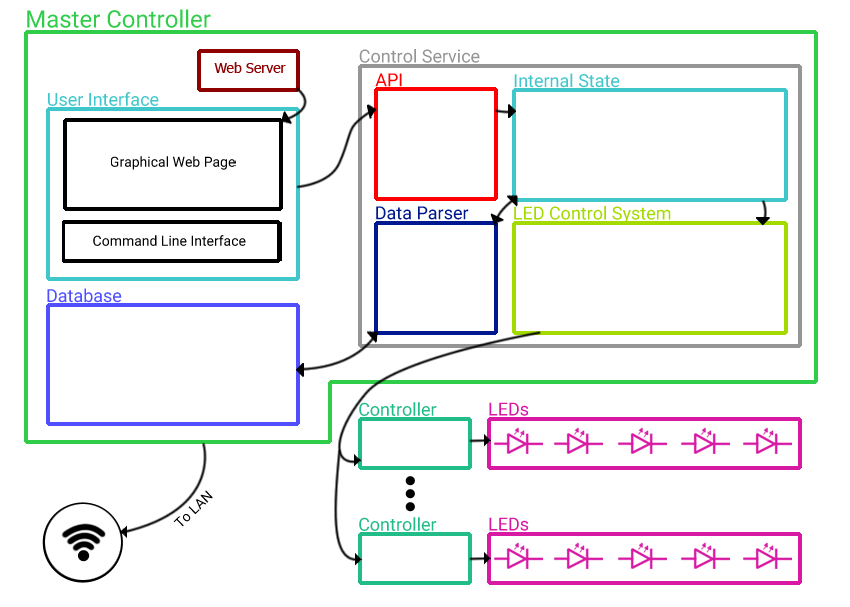
\includegraphics[width=\linewidth]{systemDiagrams/systemdiag.png}
				\caption{The PlanteR-GB system including interface and control systems}
				\label{fig:systemDiagram}
			\end{figure}
		\end{center}

		\subsection{Hardware}
			\subsubsection{Overview}
			\subsubsection{Master Controller}
			\subsubsection{LED Controller(s)}
			\subsubsection{LED strips}


		\subsection{Control Service}
			\subsubsection{Overview}
			The control service is the bridge between the user interface and the LEDs.
			It has an API that serves as the entry point for all system changes, an internal state representation which is fed to the LED control system and also translated into persistent storage.
			The API obfuscates the communication between the client UI and the control service by providing a set of routes through which data can be sent.
			To make a data request or modification, the client sends data to the control service using one of the REST verbs (GET, POST, PUT, DELETE, etc).
			Using the REST protocol simplifies communication between client and server, but also allows new settings and parameters to quickly become accessible through the addition of new routes.

			\noindent \\The control service internal state is the primary representation of the configuration and settings of the system.
			This internal state is the focal point of the API, data storage, and LED control system.
			It is responsible for representing all data and committing it into persistent storage.
			When a client UI makes a change to a system parameter, the data is routed through the API and into the internal state.

			\noindent \\The data parser is responsible for translating the system state into persistent storage when changes are made.
			When the system starts, the data parser reads from persistent storage and rebuilds the internal state.
			A database with tables closely mirroring the internal state objects is the persistent end of the data parser.

			\subsubsection{API}
			%pistache.io is a good REST library for C++
			The API implements a REST protocol. REST is an architectural style and modern approach to web service communication. \cite{rest1}
			It provides a lightweight communication protocol between client and server, making it a popular building style for cloud-based APIs.
			The control service API consists of a series of routes, each relevant to a particular parameter or set of parameters.
			The internal state is updated when a client sends a request to the API.

			\noindent \\Here is an example of a series of REST requests which build a basic functioning system:
			\begin{lstlisting}[language=XML]
// Create an LED state with ID 3
PUT http://localhost:5324/ledstate/3
// Set the color of LED state 3 to red
POST http://localhost:5324/ledstate/3/color/ff0000
// Set the intensity of LED state 3 to 85%
POST http://localhost:5324/ledstate/3/intensity/85
// Set the power of LED state to on
POST http://localhost:5324/ledstate/3/power/on

// Add a new schedule with ID 4
PUT http://localhost:5324/schedule/4/
// LED state 3 triggers at 8:30am
POST http://localhost:5324/schedule/4/hour/0830/ledstate/3
// LED state 4 triggers at 2:00pm
POST http://localhost:5324/schedule/4/hour/1600/ledstate/4
// LED state 0 triggers at 9:00pm
POST http://localhost:5324/schedule/4/hour/2100/ledstate/0

// Add a new zone with ID 3
PUT http://localhost:5324/zone/3/
// Set the schedule used by zone 3 to schedule 4
POST http://localhost:5324/zone/3/schedule/4
// Assign LEDs 1 through 4 to zone 3
POST http://localhost:5324/zone/3/leds/1-4
// Assign LEDs 6 through 8 to zone 3
POST http://localhost:5324/zone/3/leds/6-8
// Assign LED 9 to zone 3
POST http://localhost:5324/zone/3/leds/9

// Get the current color of zone 3
GET http://localhost:5324/zone/3/color/

// Delete zone 3
DELETE http://localhost:5324/zone/3/
\end{lstlisting}

			\subsubsection{Internal State}
			The internal state of the system is represented by a series of objects closely mirroring their physical counterparts.
			An object is a template that can be instantiated into memory, and then manipulated.
			Using objects allows the system to represent its properties in a human readable way, as well as easily translate them into persistent storage and LED controller data.

			\noindent \\In this system, the smallest unit of measurement is the LED. The properties assigned to groups of LEDs defines the behavior of the system as a whole.
			A strip may have any number of individually controllable LEDs, attached to an LED controller.
			The Controller contains all information needed for the Control Service to locate and communicate with a physical LED controller.
			The Zone is the next highest unit of measurement, and represents a set of relationships between LEDs and a shared schedule of behavior.
			The LEDs within a zone can come from any number of LED strips attached to any LED controllers in the system.
			A schedule contains a series of time stamps each of which point to an LED state.
			Color, intensity, and power (on/off) are the three properties of an LED. An LED state defines a single combination of these properties, and can be assigned to a Zone at a specific time.


			\noindent \\This diagram shows the internal state of the control service:

			\begin{center}
				\begin{figure}[H]
					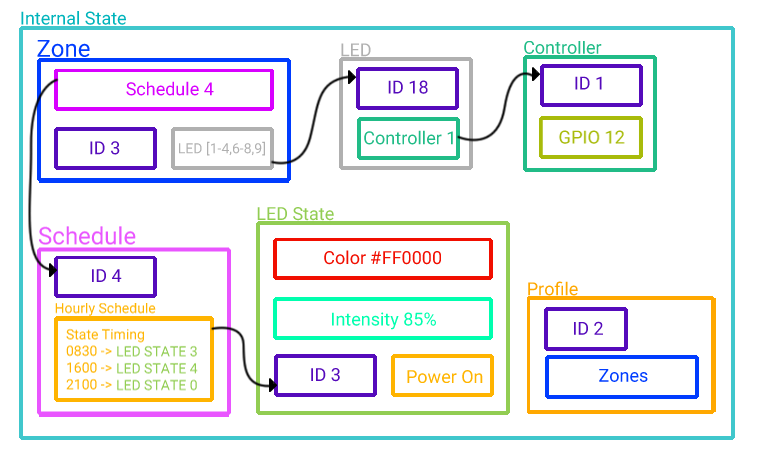
\includegraphics[width=\linewidth]{systemDiagrams/internalstate.png}
					\caption{The Internal state of the Control Service is the primary data representation, which is translated as necessary to persistent storage and LED control system.}
					\label{fig:internalStateDiagram}
				\end{figure}
			\end{center}

			\subsubsection{Data Parser}
			The data parser serves as a translator between internal state and persistent storage.
			Data flows from the Control Service API, into the internal state, and then finally to the Data Parser where the data is saved.
			The data parser has a series of functions which take internal state objects as parameters, and generate queries that are ran against the database.
			In addition to saving data, the data parser has functions that query the database and return internal state objects.
			Lastly, the data parser is responsible for any conversion routines necessary should the data format be changed significantly between iterations.


		\subsection{Data Design}
			\subsubsection{Overview}
			% Probably SQLite, because MySQL is a memory hog
			The persistent data storage is done with a database.
			The Data Parser in the Control Service translates the internal state into a series of SQL commands to INSERT, UPDATE, or DELETE from the data tables.
			A database is used because of its ability to update, delete, or read a single piece of information without requiring the entire data structure to be read into memory.
			When changes are made to the way data is structured in the internal state, the database can be restructured and updated with a short script.

			\noindent \\These are the tables that exist within the database:
			\begin{center}
				\begin{figure}[H]
					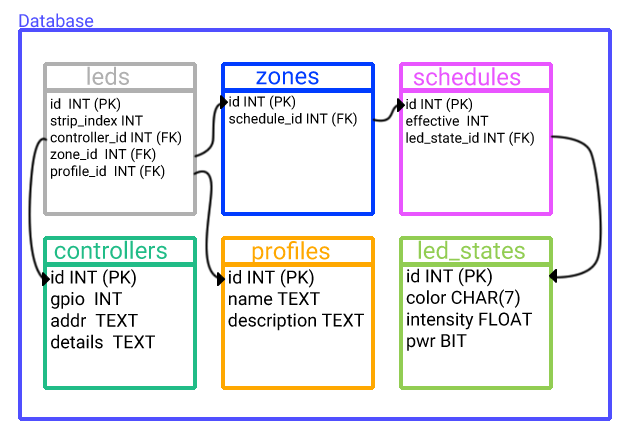
\includegraphics[width=\linewidth]{systemDiagrams/database.png}
					\caption{Schema Diagram of the database tables}
					\label{fig:databaseDiagram}
				\end{figure}
			\end{center}

			\subsubsection{Data Description}
			In the database, LEDs are stored with an ID, zone, profile, and controller. Zones store the schedule that all LEDs within it follow.
			Schedules store LED states and the time that each becomes active. LED states store color, intensity, and the power state.
			Lastly, profiles store a name and description, but each LED itself stores the Zone it belongs to per Profile.

			\noindent \\The tables below contain example data that represents how a real system might look.

			\subsubsection{LEDs table}
				\begin{tabular}{ |c|c|c|c|c| }
					\hline
					id (INT) & strip\_index (INT) & controller\_id (INT) & zone\_id (INT) & profile\_id (INT) \\
					\hline
					1 & 1 & 1 & 1 & 1 \\
					2 & 2 & 1 & 2 & 1 \\
					3 & 3 & 1 & 1 & 1 \\
					4 & 4 & 1 & 2 & 1 \\
					5 & 1 & 2 & 1 & 1 \\
					6 & 2 & 2 & 2 & 1 \\
					7 & 3 & 2 & 3 & 1 \\
					8 & 4 & 2 & 3 & 1 \\
					\hline
				\end{tabular}

			\subsubsection{LED States table}
				\begin{tabular}{ |c|c|c|c| }
					\hline
					id (INT) & color (CHAR(7)) & intensity (FLOAT) & pwr (BIT)\\
					\hline
					1 & 000000 & 0 & 0 \\
					2 & FF0000 & 85 & 1 \\
					3 & 00FF00 & 60 & 1 \\
					4 & 0000FF & 60 & 1 \\
					\hline
				\end{tabular}

			\subsubsection{Zones table}
				\begin{tabular}{ |c|c| }
					\hline
					id (INT) & schedule\_id (INT) \\
					\hline
					1 & 1 \\
					2 & 1 \\
					3 & 2 \\
					\hline
				\end{tabular}

			\subsubsection{Schedules table}
				\begin{tabular}{ |c|c|c| }
					\hline
					id (INT) & effective (INT) & led\_state\_id (INT) \\
					\hline
					1 & 800 & 2 \\
					1 & 1800 & 1 \\
					2 & 430 & 3 \\
					2 & 934 & 4 \\
					2 & 2200 & 1 \\
					\hline
				\end{tabular}

			\subsubsection{Profiles table}
				\begin{tabular}{ |c|c|c| }
					\hline
					id (INT) & name (TEXT) & description (TEXT) \\
					\hline
					1 & ``Default'' & ``The default schedule that happens every day'' \\
					2 & ``Holiday'' & ``Lights flash green and red for 30 minutes in the morning, then return to normal'' \\
					2 & ``Vacation'' & ``Lights come on earlier in the morning and turn off later'' \\
					\hline
				\end{tabular}

			\subsubsection{Controllers table}
				\begin{tabular}{ |c|c|c|c| }
					\hline
					id (INT) & gpio (INT) & addr (TEXT) & details (TEXT) \\
					\hline
					1 & 26 & ``NULL'' & ``NULL'' \\
					2 & 17 & ``NULL'' & ``NULL'' \\
					3 & 0 & ``DF:48:16:A3:44:2B'' & ``protocol:3'' \\
					\hline
				\end{tabular}


		\subsection{LED Control System}
			\subsubsection{Overview}
			\subsubsection{LED Controller Communication}
			\subsubsection{LED Controller Software}

		\subsection{Stretch goal: Custom Enclosure}
			\subsubsection{Overview}
		\subsection{Stretch goal: External sensors}
			\subsubsection{Overview}

			\section{Human Interface Design}
			        \subsection{Overview of User Interface}
			        They way humans interface with a program is an important part of any program.
			        For this project there will be two iterations of the human interface. The
			        first being over command line. The second would be through a web interface.
			        \subsection{Command Line Interface}
			            \subsubsection{Interface Overview}
			            The command line interface will ask questions of the user about how they
			            would like to configure the settings. There will be 5 options for them to
			            choose from in the main menu. Those options are, Bed Options, Zoning Options,
			            Scheduling Options, Profile Options and the final option is to apply changes.
			            Each Option as sub options to configure that section. For example in the
			            scheduling section it will prompt you to edit a schedule or to add a schedule.
			            If you choose to edit a schedule you will then be taken to choose which
			            schedule you would like to modify and then you can choose all the options
			            such as what time it starts, what color you want and what brightness you would like.
			            Once all the options are filled in then it will take you back to the main
			            option page where you can apply the changes.
			            \subsubsection{Command Line Mockup}
			            \begin{center}
			                \begin{figure}[H]
			                    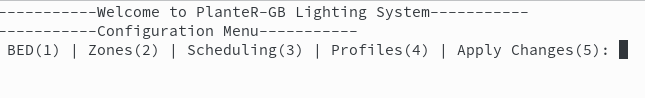
\includegraphics[width=\linewidth]{comand_line_interface/Selection_006.png}
			                    \caption{Start of Command Line Interface}
			                    \label{fig:Start of Command Line Interface}
			                \end{figure}

			                \begin{figure}[H]
			                    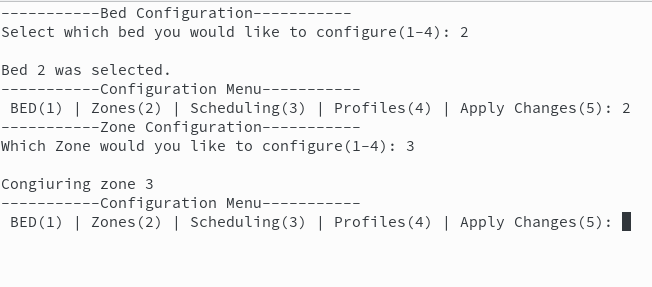
\includegraphics[width=\linewidth]{comand_line_interface/Selection_003.png}
			                    \caption{Bed and Zone Selection Menu}
			                    \label{fig:Bed and Zone Selection Menu}
			                \end{figure}

			            \begin{figure}[H]
			                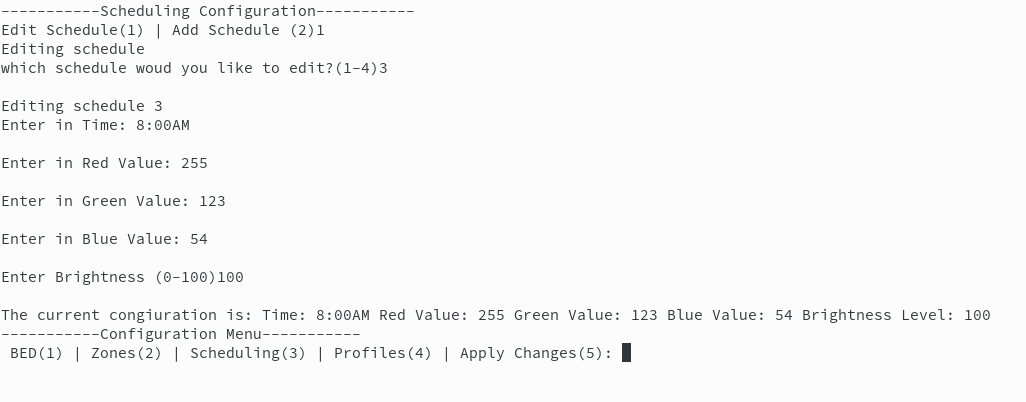
\includegraphics[width=\linewidth]{comand_line_interface/Selection_004.png}
			                \caption{Scheduling Configuration Menu}
			                \label{fig:Scheduling Configuration Menu}
			            \end{figure}

			            \begin{figure}[H]
			                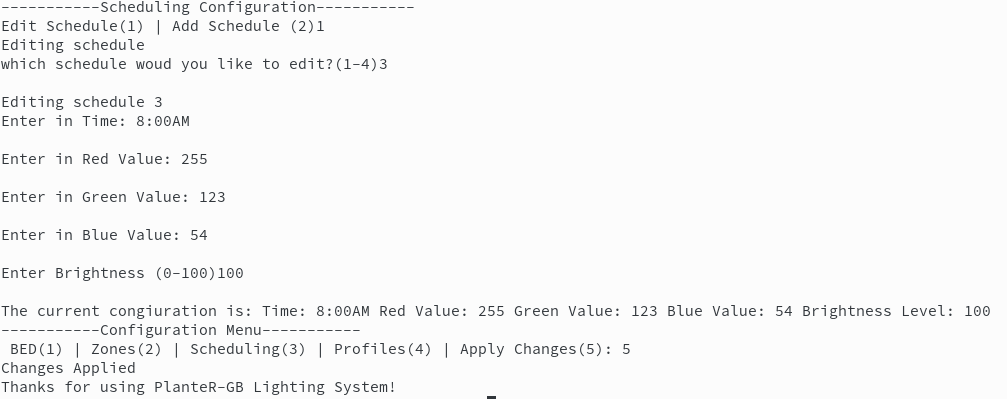
\includegraphics[width=\linewidth]{comand_line_interface/Selection_005.png}
			                \caption{End of Command Line Interface}
			                \label{fig:End of Command Line Interface}
			            \end{figure}
			        \end{center}

			        \subsection{Web Interface}
			            \subsubsection{Interface Overview}
			            The web interface will consist of four pages to configure the settings of
			            the lighting system. The pages are the home page where the bed that the user
			            wishes to modify is selected. The Zoning page where the user can select
			            the zones the user would like to set on the LED strips. A Scheduling page
			            to set up schedules for when to turn on and off, what color and how bright.
			            The last page is the profile page where a user can create and change profiles.
			            The currently selected bed and profile will appear in the top right corner.
			            Below each page will be discussed in more detail and a mockup of each page
			            is displayed.
			            \subsubsection{Home Page}
			            The home page of the web interface will prompt the user to select which
			            bed they would like to modify. If the user only has one bed hooked up there
			            will only be one option. If more beds are added it will add more beds to this
			            section. The chosen bed will appear in the top right corner under Currently
			            Selected.
			            \subsubsection{Home Page Mockup}
			            \begin{center}
			                \begin{figure}[H]
			                    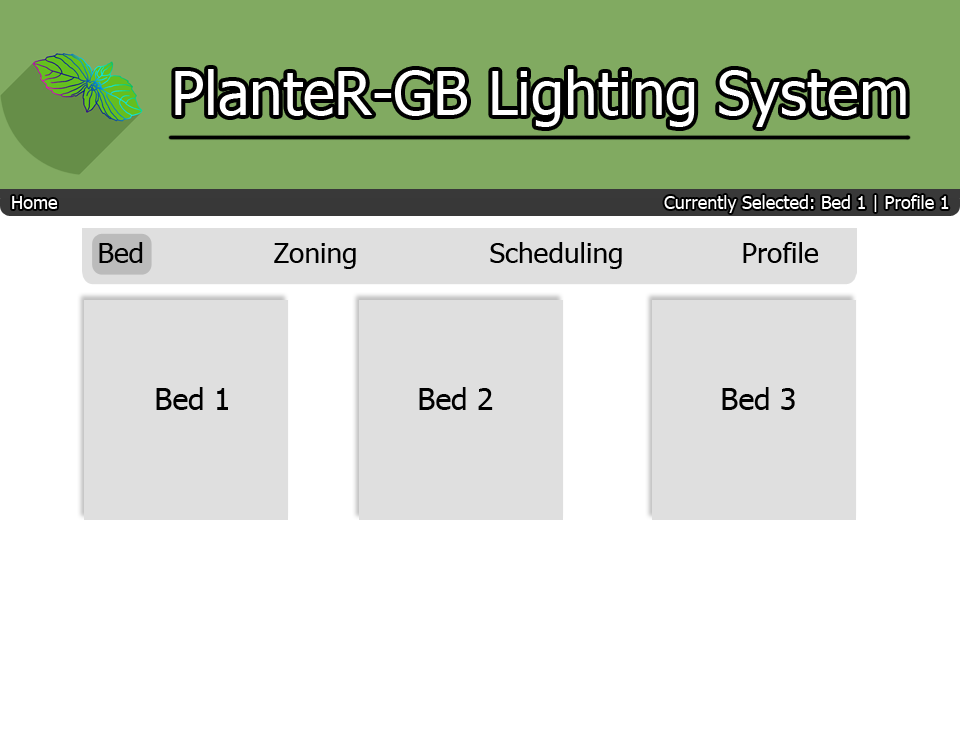
\includegraphics[width=\linewidth]{web_design/BedPage.png}
			                    \caption{Home Web Page}
			                    \label{fig:Home Page}
			                \end{figure}
			            \end{center}
			            \subsubsection{Zones Page}
			            The zoning section of the web page will be where they user sets zones on
			            the LEDs. It will show the user all the LED strips that are on that bed
			            and will allow them to assign each LED to a zone by click on it. The number
			            of zones can be added to by clicking the "Add Zone" button. They will appear
			            below with the color that is assigned to that zone. You can then select
			            which zone you would like to add LEDs too by clicking the drop down menu "Select Zone".
			            When you add an LED to a zone a box with that color will appear around it
			            and grow as more LEDs are added to the zone.
			            \subsubsection{Zoning Page Mockup}
			            \begin{center}
			                \begin{figure}[H]
			                    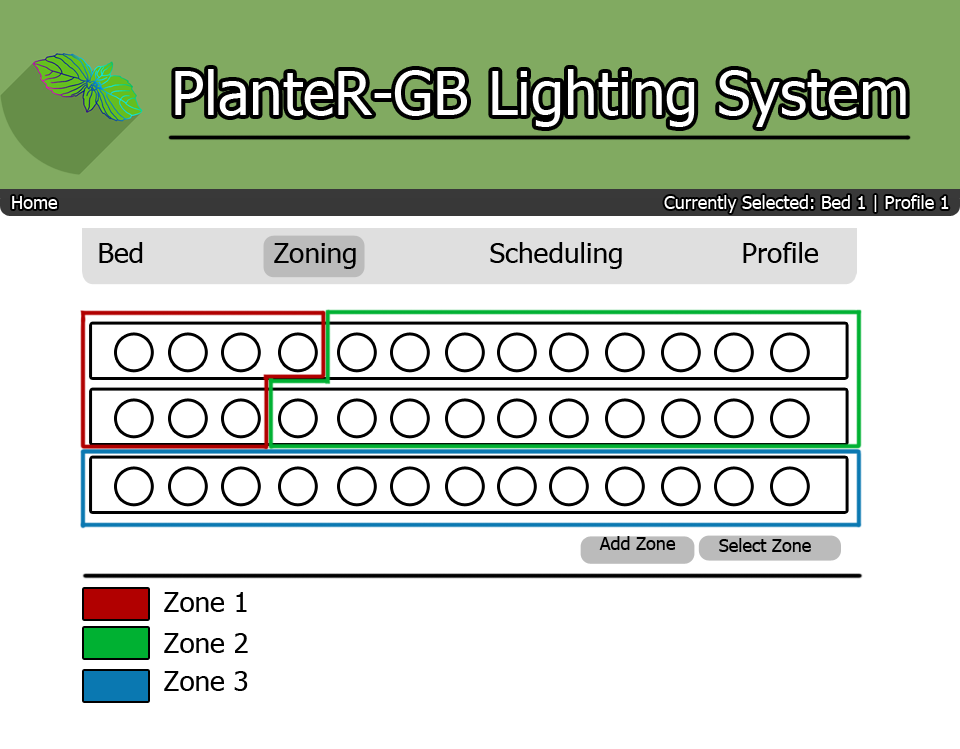
\includegraphics[width=\linewidth]{web_design/ZoningPage.png}
			                    \caption{Zoning Web Page}
			                    \label{fig:Zoning Page}
			                \end{figure}
			            \end{center}
			            \subsubsection{Schedule Page}
			            The schedule page will be where the main part of the configuration is done.
			            This is where you would select what time color and brightness of the LEDs.
			            You can have different schedules for different zones. You can add new schedule
			            by clicking the "Add Schedule" button and it will add a new schedule to the
			            list.
			            \subsubsection{Schedule Page Mockup}
			            \begin{center}
			                \begin{figure}[H]
			                    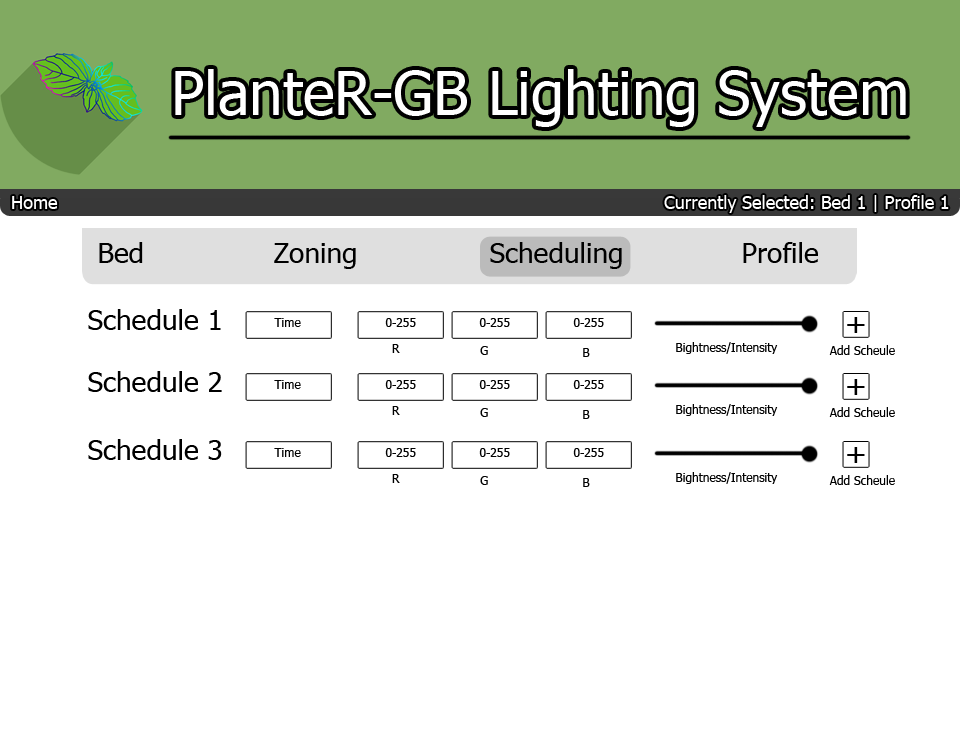
\includegraphics[width=\linewidth]{web_design/SchedulingPage.png}
			                    \caption{Scheduling Web Page Mockup}
			                    \label{fig:Schedule Page}
			                \end{figure}
			            \end{center}
			            \subsubsection{Profile Page}
			            The profile page is where you can switch or create new profiles. The profile
			            that is currently selected is in the top right of the screen under the "Currently
			            Selected" section.
			            \subsubsection{Profile Page Mockup}
			            \begin{center}
			                \begin{figure}[H]
			                    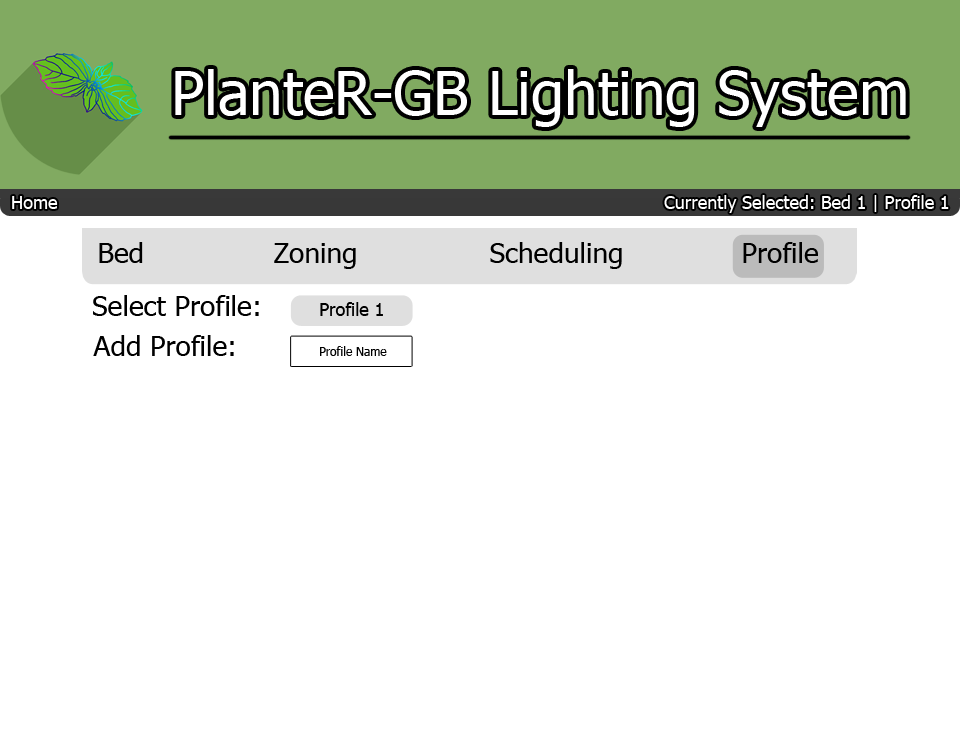
\includegraphics[width=\linewidth]{web_design/ProfilePage.png}
			                    \caption{Profile Web Page Mockup}
			                    \label{fig:Profile Page}
			                \end{figure}
			            \end{center}


	% Scheduling
	\section{Project Timeline}
		\subsection{Iteration 1}
		\subsection{Iteration 2}
		\subsection{Iteration 3}
		\subsection{Iteration 4}
		\subsection{Iteration 5}
		\subsection{Iteration 6}

	%\section{Requirements Matrix} %??? What is this, it was in a template somewhere

	\section{Appendices} % OR glossary??



\end{document}
